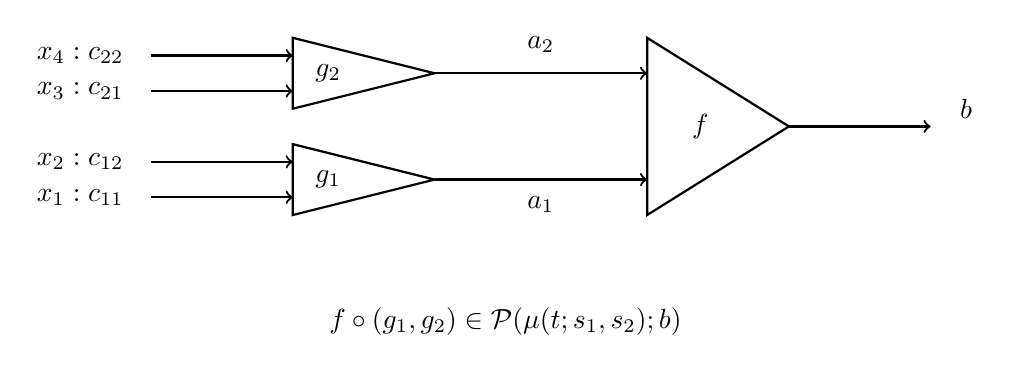
\begin{tikzpicture}[scale=0.9]
    % Main operation triangle
    \draw[thick, fill=white] (0,0) -- (0,2.5) -- (2,1.25) -- cycle;
    \node at (0.75,1.25) {$f$};

    % First sub-operation triangle
    \draw[thick, fill=white] (-5,0) -- (-5,1) -- (-3,0.5) -- cycle;
    \node at (-4.5,0.5) {$g_1$};

    % Second sub-operation triangle
    \draw[thick, fill=white] (-5,1.5) -- (-5,2.5) -- (-3,2) -- cycle;
    \node at (-4.5,2) {$g_2$};

    % Input arrows for first sub-operation
    \draw[->, thick] (-7,0.25) -- (-5,0.25);
    \draw[->, thick] (-7,0.75) -- (-5,0.75);
    \node at (-8,0.25) {$x_1: c_{11}$};
    \node at (-8,0.75) {$x_2: c_{12}$};

    % Input arrows for second sub-operation
    \draw[->, thick] (-7,1.75) -- (-5,1.75);
    \draw[->, thick] (-7,2.25) -- (-5,2.25);
    \node at (-8,1.75) {$x_3: c_{21}$};
    \node at (-8,2.25) {$x_4: c_{22}$};

    % Connecting arrows from sub-operations to main operation
    \draw[->, thick] (-3,0.5) -- (0,0.5);
    \node at (-1.5,0.15) {$a_1$};
    \draw[->, thick] (-3,2) -- (0,2);
    \node at (-1.5,2.4) {$a_2$};

    % Output arrow
    \draw[->, thick] (2,1.25) -- (4,1.25);
    \node at (4.5,1.5) {$b$};

    % Final composition label
    \node at (-2,-1.5) {$f \circ (g_1, g_2) \in \mathcal{P}(\mu(t; s_1, s_2); b)$};

\end{tikzpicture}